% !TEX root = Case.tex

\subsection*{About the applicants}
\noindent 
The applicants have found (UGe$_2$, URhGe, UAu$_2$)
%We have discovered the first Fe-based superconductor without chalcogenide and pnictide elements, YFe$_2$Ge$_2$ \citesel{chen16}, the only Fe-based superconductor discovered in the UK and one of only a handful that were discovered in Europe. This was recently followed up by the discovery of superconductivity in LuFe$_2$Ge$_2$.
\paragraph{Malte Grosche (FMG)} 
is head of the Quantum Matter
group at the Cavendish Laboratory, with a 25 year track record of quantum materials research, which includes all the projects mentioned above. 
%Highlights include the realisation of the key role of magnetic quantum critical points for inducing unconventional superconductivity in CePd$_2$Si$_2$ and CeIn$_3$ \citesel{mathur98}, the first superconducting band ferromagnet UGe$_2$ \citesel{saxena00}, two-dome superconductivity in Ge-doped CeCu$_2$Si$_2$ \citesel{yuan03}, exploiting the tunability of electronic and phonon spectrum in superconducting clathrates \citesel{grosche01a}), quasi-skutterudites \citesel{klintberg12, goh15} and quasiperiodic materials \citesel{brown18}, and now the discovery and investigation of unconventional superconductivity in YFe$_2$Ge$_2$ \citesel{chen16,chen20b} and in the high-pressure structure of CeSb$_2$. 
Other recent projects feature %the discovery of unconventional superconductivity in YFe$_2$Ge$_2$ \citesel{chen16}, the demonstration that low-lying sliding modes specific to quasiperiodic materials foster strong-coupling superconductivity in high pressure bismuth \citesel{brown18}, 
quantum oscillation measurements in the pressure-metallised Mott insulator NiS$_2$ % by
% quantum oscillation measurements
\citesel{friedemann16,semeniuk22} (\autoref{fig:Highlights}), and the identification of quantum tricritical points in the band magnet NbFe$_2$ \citesel{friedemann18}. %, and the discovery of a structural quantum critical point in Ca$_{3}$Ir$_4$Sn$_{13}$ and Ca$_3$Rh$_4$Sn$_{13}$  \citesel{klintberg12,goh15}. 
His publications 
%include three Nature and Science papers (e.g. \citesel{yuan03}) and 
have attracted over 5,500
citations. 
FMG will coordinate the overall management of this project, liaise with project partners, and oversee materials selection, data analysis and dissemination of results. 


% Recent work includes the demonstration of a marginal Fermi liquid state in NbFe$_2$
% \citesel{brando08} and the discovery of a pressure-induced superlattice quantum critical
% point in the quasi-skutterudite Ca$_3$Ir$_4$Sn$_{13}$ \citesel{klintberg12}.

%\paragraph {James Annett (JFA)} is ...  

\paragraph{Mike Sutherland (MLS)}
is an Affiliated Lecturer and Fellow of Corpus Christi College, having previously held a
Royal Society University Research Fellowship. MLS has 20 years experience in precision transport and
magnetic measurements at low temperatures and in high magnetic fields (e.g. \citesel{smith08}). Recent %research
highlights include thermal transport studies in the Kondo insulator SmB$_6$ \citesel{hartstein18}, in non-Fermi liquid materials \citesel{sutherland15,sutherland12} and in superconductors \citesel{sutherland12a,grissonnanche14}. MLS will oversee measurements in our 20.4 T cryomagnet facility and coordinate in-house and collaborative thermal transport studies.

\paragraph{Gilbert Lonzarich (GGL)}
is an Emeritus Professor and Fellow of the Royal Society, who has
made pioneering contributions in key areas of correlated electron
physics. These include (i) quantum oscillation measurements
in correlated electron systems, (ii) magnetic fluctuations in metals near the threshold of magnetism and their role in facilitating superconductivity, (iii) quantum phase transitions and quantum critical phenomena. 
%His position has been guaranteed beyond retirement for the duration of
%this project.
He has been awarded the IOP Mott
medal and prize, the HP Europhysics Prize, the IOP Max Born medal, the
IOP Guthrie medal, the Royal Society Rumford medal and the Kamerlingh Onnes Prize. His publications, which include twelve in
Science and Nature, have
attracted more than 12,500 citations. Recent highlights
include studies of % the discovery of an
% the unconventional Fermi surface in % the
% topologically insulating material
%SmB$_6$
%\citesel{tan15}, % the study of 
the electronic structure
of high-$T_c$ superconductors
\citesel{hsu21,hartstein20} and % the
% theoretical and experimental investigation of
of quantum critical fluctuations in
ferroelectric materials \citesel{enderlein20,coak20}. GGL will lead on the interpretation of results and the computationally assisted search for new superconductors.

\subsection*{Other researchers}
\paragraph{Jiasheng Chen (JC)} is a postdoctoral researcher, who 
has been studying superconductivity in YFe$_2$Ge$_2$ since its discovery \citesel{zou14}. Having systematically eliminated the main causes of disorder, he produced the first high quality bulk superconducting samples \citesel{chen16}  and established a horizontal flux growth method that produces ultra-pure single crystals of YFe$_2$Ge$_2$ \citesel{chen20b}, LuFe$_2$Ge$_2$, and CeNi$_2$Ge$_2$. His transport and heat capacity measurements suggested that superconductivity in YFe$_2$Ge$_2$ is unconventional \citesel{chen19}, and he has already led preliminary neutron and $\mu$SR studies. 
%As part of his work on metallic magnetocalorics, JC has developed a 60 mK refrigeration module for the Quantum Design PPMS, which will be used in this project. 
JC will be in charge of crystal growth and characterisation and will take a central role in measurements at large facilities.

%\paragraph{Thomas Gruner (TG)} is a Humboldt-Society Feodor Lynen
%fellow at the Cavendish Laboratory, who has pioneered intermetallic
%compounds for adiabatic demagnetisation refrigeration at low
%temperature \citesel{gruner14,jang15}.  TG has nine years experience in
%synthesis and characterisation of challenging materials
%\citesel{gruner17} and will oversee the cuprate crystal growth
%%gruner10,
%facility.

\paragraph{Puthipong Worasaran (PW)} has in late 2021 finished his PhD in our group, during which he demonstrated outstanding expertise in challenging transport and magnetic measurements in anvil-cell devices at hydrostatic pressures exceeding $\SI{100}{\kilo\bar}$. He will be in charge of most of the high pressure measurements.


\paragraph{Patricia Alireza (PLA)} is a senior postdoctoral researcher with 20 years experience in high pressure techniques for low temperature measurements. PLA has pioneered transport and magnetic high pressure methods, which have been taken up widely by the community. These include the introduction of miniature coils into the sample space of anvil pressure cells for susceptibility, skin depth and NMR measurements \citesel{alireza03,friedemann16,semeniuk22,meissner10}, and the construction of ultra-low-background miniature anvil cells for use in commercial SQUID magnetometers \citesel{alireza09a,alireza09}, which enabled the detection of the Meissner effect in high pressure hydrogen sulfide by the Eremets group. %\citesel{drozdov15}.
%By introducing miniature coils into the sample space of anvil pressure cells, she enabled high precision magnetic susceptibility measurements \citesel{alireza03} and paved the way for high frequency skin depth \citesel{friedemann16} and NMR measurements \citesel{meissner10} in anvil cells. She constructed an ultra-low-background miniature anvil cell for use in commercial SQUID magnetometers \citesel{alireza09a}, which facilitates the rapid scanning of superconducting phase diagrams \citesel{alireza09b}. 
PLA oversees high pressure development and trains incoming graduate students.
  
%{\em Richard Needs, Claudio Castelnovo and Johannes Knolle} from the Theory of Condensed Matter group at the Cavendish
%Laboratory, Cambridge and {\em Dmitry Kovrizhin} from the Centre for Theoretical
%Physics, Oxford, who contribute wide-ranging expertise in numerical
%and analytic studies of correlated systems; \\

%\paragraph{Ivan Kokanovic}


\begin{figure}
 {\em Relevant publications by the participating researchers} 

\vspace{0.5em}

\begin{tabular*}{0.98\columnwidth}{|@{\hspace{0.5em}}
    p{0.52\columnwidth} @{\extracolsep\fill} 
    p{0.38\columnwidth}@{\hspace{0.5em}}|}
\hline
% {\em Topic area} & {\em References} \\
% \hline\hline
Discovery & \citesel{mathur98,saxena00,grosche00,klintberg12,zou14,chen16} \\
High quality crystal growth & \citesel{friedemann16, friedemann18,  chen19, chen20b} \\ %rourke10
Tuning by pressure or chemical substitution &
\citesel{yuan03,chen16,friedemann18,goh15,alireza09,klintberg12}
\\
Quantum oscillation, transport or
  thermodynamic measurements &\citesel{hartstein18,friedemann16,semeniuk22,sutherland15,hartstein20,hsu21,sutherland12, sutherland12a,grissonnanche14,goh08,smith08,baglo21} \\ %,kokanovic09,yelland08,storey13} \\
Technical developments & \citesel{alireza03,alireza09a,alireza09,meissner10,friedemann16}\\ %,storey13,welzel11}\\
%citesel{duncan10,sutherland11,loram83,saha14,tallon11,goh12,bartlett15}
\hline
\end{tabular*}

\vspace{1em}

\centerline{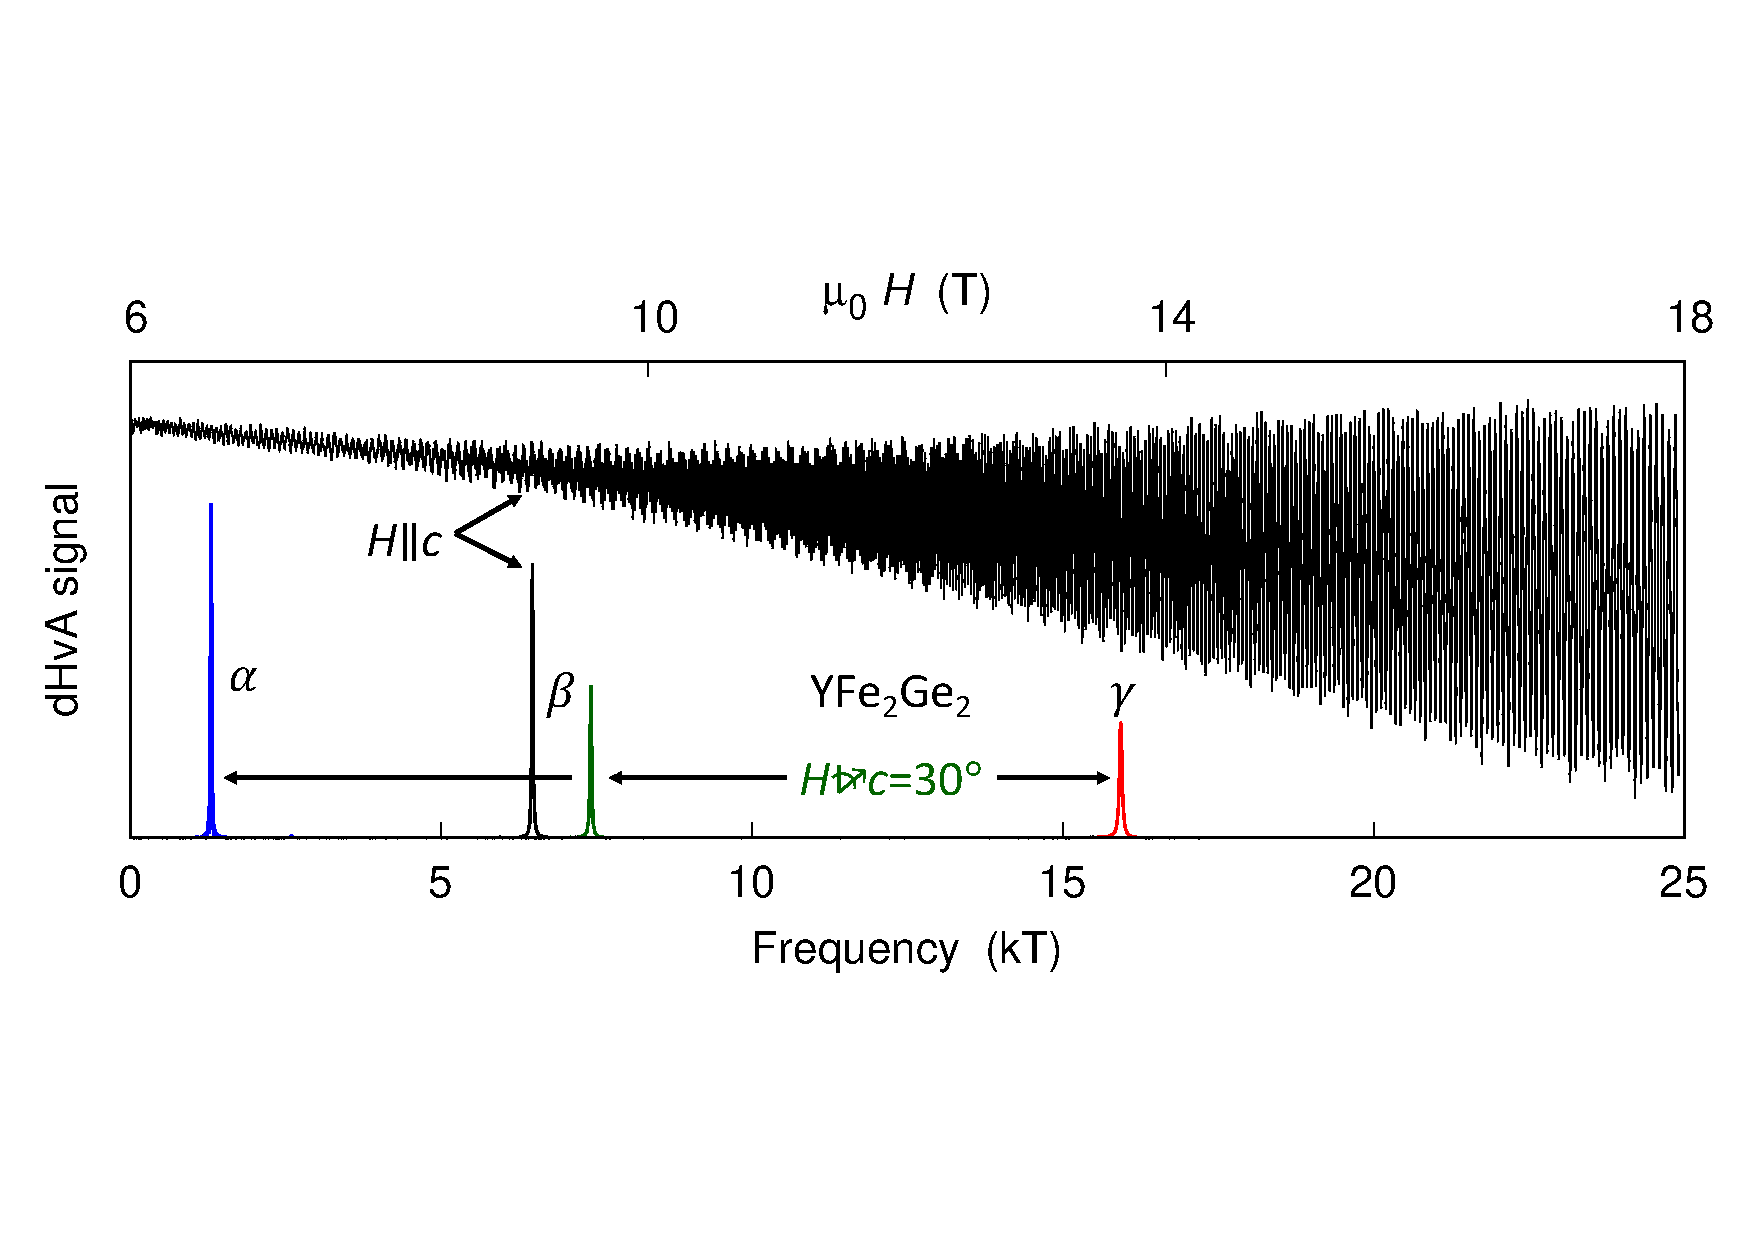
\includegraphics[width=\columnwidth]{Figures/YFGQOPlotFig}}
\centerline{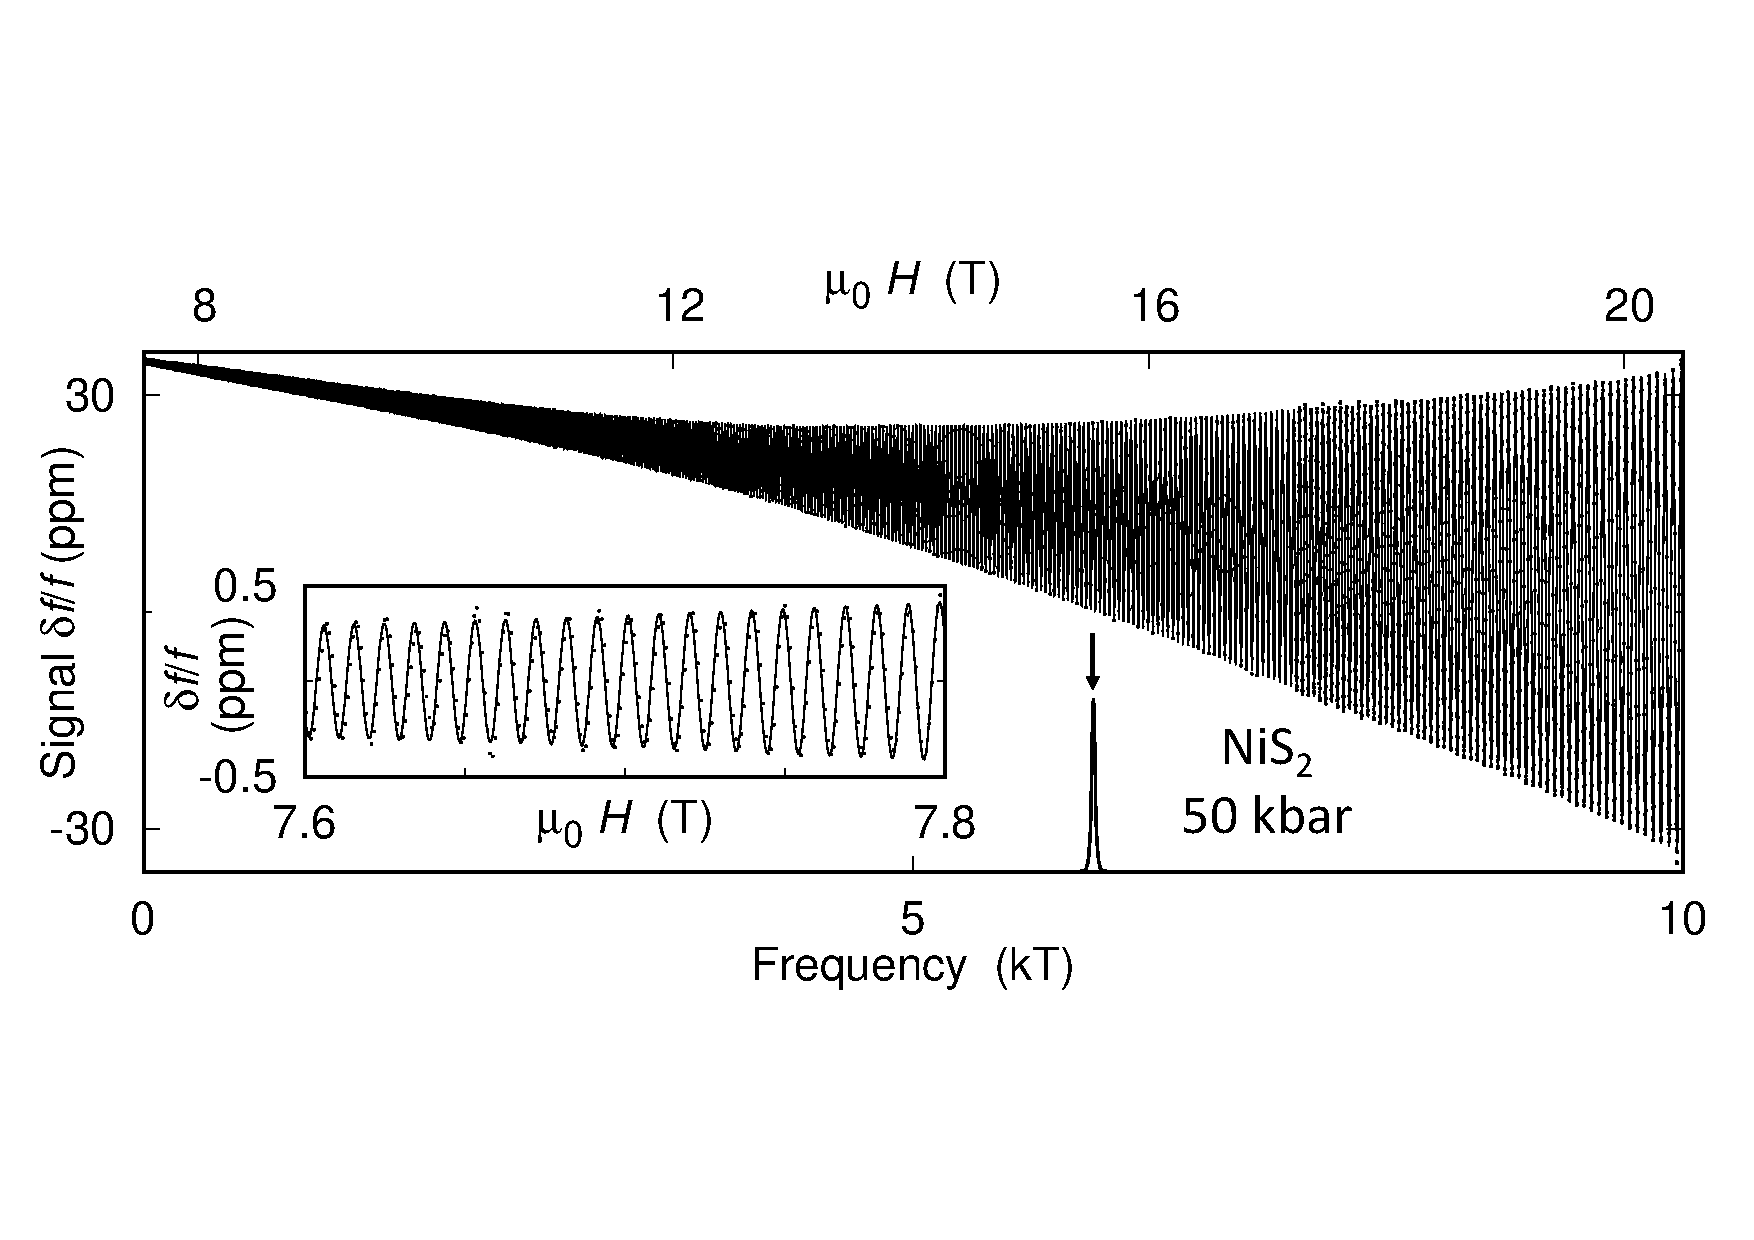
\includegraphics[width=\columnwidth]{Figures/NiS2QOPlotFig}}
 %\centerline{\includegraphics[width=0.75\columnwidth]{\Figures/Pressure/HighPQuantOsc/Ca2RuO4.pdf}}
\caption{{\bf Recent highlights:} The table lists selected
  publications in relevant areas. The figures show quantum oscillations signals recorded in the unconventional superconductor YFe$_2$Ge$_2$ (upper panel) \protect\citesel{baglo21} and in the correlated metallic state on the  threshold of Mott localisation in high pressure NiS$_2$ (lower panel) \protect\citesel{friedemann16,semeniuk22},
%  In both cases, the signal can be resolved down to  
%magnetic fields less than $8~\text{T}$
resolving key aspects of the electronic structure and demonstrating the high quality of in-house-grown crystals. }%The oscillation  frequencies give the extremal cross-sectional area of  the Fermi surface. 
%  The effective carrier mass, renormalised by interactions, can be derived from the temperature dependence of the oscillation amplitude. 
%  The high pressure data was obtained by tracking the  resonance frequency of an $LC$ oscillator, with the resonance coil  inside the sample volume of an anvil pressure cell \protect\citesel{semeniuk22}.}
\label{fig:Highlights}
\end{figure} 



% Moreover, the work will benefit from c
\subsection*{Key project partners} 
%{\em Geetha Balakrishnan}, Professor at the University of Warwick
% specialises in the growth of single crystals of superconductors and related magnetic materials. She will provide guidance and support on aspects of materials preparation for some of the systems, for example the rare earth hexa- and dodecaborides and skutterudites (objectives 1,3,4-7).

%{\em Alix McCollam}, Professor at Radeboud University and staff scientist at HFML Nijmegen ... \\
\paragraph{Antony Carrington, Sven Friedemann,} University of Bristol, will carry out penetration depth measurements using the tunnel-diode oscillator technique at ambient and elevated pressure and pursue transport and Raman measurements to ultra-high pressures.%electrical transport, neutron and x-ray studies on Cambridge-grown cuprate crystals. 

\paragraph{Devashibhai Adroja,} Rutherford Appleton Laboratory, will lead on muon spin rotation and neutron scattering studies of superconducting and magnetic states as well as magnetic excitations.

%\paragraph{Ingo Loa,} CSEC Edinburgh, will collaborate on high pressure structure determination using synchrotron x-ray sources.
%\paragraph {Juri Grin, Andrew Mackenzie, Manuel Brando,} MPI for Chemical Physics of Solids (Dresden/Germany), will analyse crystal quality by x-ray crystallography, SEM, TEM and other microscopic probes and carry out low temperature thermodynamic and dilatometric measurements.

\paragraph{Andrey Chubukov,} University of Minnesota, will contribute wide-ranging expertise in numerical
and analytic studies of quantum materials and help with interpreting experimental results. 


%{\em Monika Gam{z}a}, Lecturer at the University of Central
%Lancashire with long-standing expertise in crystal growth and crystallography, will carry out detailed characterisation by single crystal x-ray diffraction.
% . MG will bring expertise in careful characterisation measuresurements of single crystal samples, in particular using magnetisation \citesel{svanidze_itinerant_2015} and x-rays \citesel{gamza_electronic_2014}. Sample characterisation is especially important for studies in systems near phase transitions, as inhomogeneities can mask trends in tuning studies (objectives 1,3,4-7).


 




\subsection*{Research environment and prior work}
\noindent
The programme benefits from substantial prior work %on advanced measurement and cooling techniques 
(\autoref{fig:Highlights}) and from sustained investment
in modern research equipment, which includes a newly upgraded 20.4~T/dilution refrigerator high field
facility, a 15~T/300~mK cryomagnet, and a
7~T/100~mK cryogen-free demagnetisation cryostat.  Experiments demanding still higher
magnetic fields will be taken to international facilities, where we
have successfully bid for magnet time in the recent past (nine weeks since
2014). Two more weeks of magnet time at HFML Nijmegen have already been granted for work on this project. % For thermopower and
% thermal conductivity below 1K, we would mainly employ our 7~T/100~mK
% cryogen-free demagnetisation cryostat, and our 300mK Helium-3
% immersion probe.
A 9~T PPMS and a 7~T SQUID
magnetometer, both equipped with Helium-3 inserts, are available for sample
characterisation and rapid turnover measurements. %  A further
% 1~T/50~mK demagnetisation cyrostat is available for work at low
% magnetic fields. 
%  A 9T PPMS with Helium-3 insert and a 7T SQUID magnetometer
% with Helium-3 insert are available for sample characterisation and for
% quick high pressure measurements. A further 1T/50mK demagnetisation
% cyrostat is available for preliminary measurements. 
Crystal growth facilities include %UHV-compatible radio-frequency induction furnaces,
two arc furnaces and a mirror furnace as well as numerous box and tube
furnaces for flux and vapour transport growth. High-quality crystals of key materials in recent studies,
such as NiS$_2$ and YFe$_2$Ge$_2$, were produced in our group
(\autoref{fig:Highlights}).  
%Most of these facilities have been
%acquired % or upgraded
%over the last decade, demonstrating the commitment of the Cavendish
%Laboratory. % to this area of research.
Advanced electron-microscopy and x-ray characterisation
equipment as well as focused ion beam facilities are available within
the Cavendish, and we can access additional growth and
characterisation facilities at the new Henry Royce Institute for
Materials in Cambridge.



% Recent achievements (Fig.~\ref{Highlights}) include
% (i) discoveries made by tuning correlated systems near quantum phase
% transitions, (ii) high precision quantum oscillation, transport  (Fig.~\ref{ThermalCond}) or
% thermodynamic measurements at low temperature, in high magnetic
% field, and under applied pressure, 
% (iii) development of new techniques such as high pressure microcoil
% de Haas-van Alphen, NMR or
% tunnel diode measurements, high pressure
% SQUID magnetometry, and patterned
% anvil cells. 
% Members of the QM group have a proven track record of developing
% bespoke, precision instrumentation for the most demanding cryogenic
% measurements. Notable successes include the design and construction of
% diamond anvil and piston cylinder cells using micro pickup coils for
% quantum oscillation measurements under pressure \citesel{goh08},
% and the construction of a thermal transport stage for high resolution
% measurements at T~$<$~4~K \citesel{smith08}.
% Moreover, materials growth work carried out over the past year as part of an EPSRC
% Impact Acceleration Grant has established the procedures for producing large pills
% of metallic magnetocalorics, a central ingredient for the envisaged compact, robust and efficient
% sub-Kelvin adiabatic demagnetisation refrigerators.
%  through the manufacture of large scale
% samples of metallic magnetocalorics.
% Through this programme we have
% developed an understanding of the growth of samples of metallic
% refrigerants, which will inform the materials preparation aspects of
% our research plan.

\vspace{-1em}

\bibliographystylesel{apsrevFMG}

\bibliographysel{References}

% \end{document}

%%% Local Variables:
%%% mode: latex
%%% TeX-master: "Case"
%%% End:
